% contenu du fichier : chap4.tex
\chapter{Émergence de la propriété petit-monde dans le modèle petit-monde}
%\newcommand{\nl}{$n_{\ell}$ } 
L'émergence de la propriété petit-monde dans le modèle Newman-Watts est encore un phénomène pas bien compris, parmi ses problématiques on cite: à partir de quel point ce réseau change sa nature grand-monde vers petit-monde ? Si ce réseau se sature par les raccourcis ajoutés, comment et quand la saturation se réalise ? Est-ce-qu'il y a vraiment une transition de phase ou non ? Etc.
Par des études théoriques confirmant par une intense nombre de simulations, on abordera quelques questions de ce genre.
\section{Introduction}

Le modèle de Watts-Storogatz (WS) connaît une attention énorme depuis son apparition en 1998 \cite{Watss-Strogatz1998}, il a deux propriétés très intéressantes: la présence d'un coefficient de Clustering élevé et d'un petit PCC. Ces deux propriétés se trouvent dans la plupart des réseaux réels \cite{Cohen-Havlinl2010,Newman2010}, en plus ce modèle est très simple et combine la régularité avec l'aléatoire. En $1999$ Newman et Watts \cite{Newman-Watts1999} ont réalisé une petite modification sur le modèle WS, dont il y a $n$ nœuds qui se distribuent dans un réseau régulier unidimensionnelle sous forme d'une cercle où chaque nœud fait $2k$ liens avec ses plus proches voisins (voir Fig.\ref{NW}), le nombre de nœuds reste fixe puis chaque lien se reconnecte par une probabilité $\phi$ entre deux autres nœuds choisis aléatoirement sans supprimer aucuns liens, les liens ajoutés sont nommé raccourcis, en moyenne il y a $x=nk\phi$ raccourcis. Ce modèle aussi connaît une grande attention car il a les m\^{e}mes propriétés du modèle WS, sauf pour $k=1$ où il y a une certaine différence\footnote{Le cas $k=1$ ne nous intériorisons jamais dans ce modèle, car dans ce cas le coefficient de Clustering est zéro, alors on prend toujours $k>1$. }, au m\^{e}me temps il est moins difficile dans l'étude.

\begin{figure}[h!]
	\centering 
	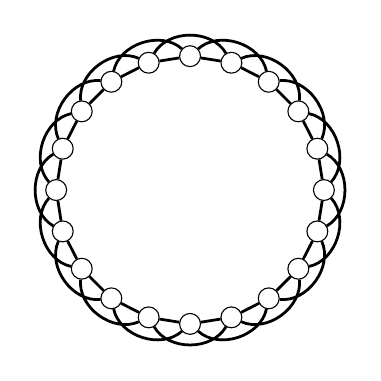
\begin{tikzpicture}[scale=0.2]
	\tikzstyle{every node}=[scale=0.4,draw,shape=circle];
	\node[scale=2]  (4) at (-18:8.5) {};
	\node[scale=2] (5) at (0:8.5) {};
	\node[scale=2] (6) at ( 18:8.5) {};
	\node[scale=2] (7) at (2*18:8.5) {};
	\node[scale=2] (8) at (3*18:8.5) {};
	\node[scale=2] (9) at (4*18:8.5) {};
	\node[scale=2] (10) at (5*18:8.5) {};
	\node[scale=2] (11) at (6*18:8.5) {};
	\node[scale=2] (12) at (7*18:8.5) {};
	\node[scale=2] (13) at (8*18:8.5) {};
	\node[scale=2] (14) at (9*18:8.5) {};
	\node[scale=2] (15) at (10*18:8.5) {};
	\node[scale=2] (16) at ( 11*18:8.5) {};
	\node[scale=2] (17) at (12*18:8.5) {};
	\node[scale=2] (18) at (13*18:8.5) {};
	\node[scale=2] (19) at (14*18:8.5) {};
	\node[scale=2] (r) at (15*18:8.5) {};
	\node[scale=2] (1) at (16*18:8.5) {};
	\node[scale=2] (2) at (17*18:8.5) {};
	\node[scale=2] (3) at (18*18:8.5) {};
	\draw[line width=1pt](r)--(1)
	(1) -- (2)
	(2) -- (3)
	(3) -- (4)
	(4) -- (5)
	(5) -- (6)
	(6) -- (7)
	(7) -- (8)
	(8) -- (9)
	(9) -- (10)
	(10) -- (11)
	(11) -- (12)
	(12) -- (13)
	(13) -- (14)
	(14) -- (15)
	(15) -- (16)
	(16) -- (17)
	(17) -- (18)
	(18) -- (19)
	(19) -- (r);
	\draw[line width=1pt] (r) to [bend right=60] (2) 
	(2)to [bend right=60](4)
	(4)to [bend right=60](6)
	(6)to [bend right=60](8)
	(8)to [bend right=60](10)
	(10)to [bend right=60](12)
	(12)to [bend right=60](14)
	(14)to [bend right=60](16)
	(16)to [bend right=60](18)
	(18)to [bend right=60](r)
	
	(1)to [bend right=60](3)
	(3)to [bend right=60](5)
	(5)to [bend right=60](7)
	(7)to [bend right=60](9)
	(9)to [bend right=60](11)
	(11)to [bend right=60](13)
	(13)to [bend right=60](15)
	(15)to [bend right=60](17)
	(17)to [bend right=60](19)
	(19)to [bend right=60](1);
	\end{tikzpicture}
\caption{Un réseau petit-monde WS pour  $n=20$, $k=2$ sans raccourcis.}
\label{NW}
\end{figure}
\begin{sloppypar}
\section{La théorie de groupe de renormalisation et transition de phase}
\end{sloppypar}
Dans un système physique proche d'une transition de phase, les méthodes d'approximations les plus courantes s'appuyant à négliger les corrélations entre un grand nombre de particules ou plutôt entre un grand nombre de degrés de liberté, ces approximations sont valables lorsque la longueur de corrélation est petite. En pratique, on sait traiter de façon simple les corrélations à deux particules. Le problème à trois particules est déjà beaucoup plus difficile. Ce type de méthodes est voué à l'échec quand la longueur de corrélation est grande.

D'où l'idée de réduction du nombre de degrés de liberté, on cherche à établir une correspondance entre un problème de longueur de corrélation donnée et un problème de longueur de corrélation plus petite. La théorie de groupe de renormalisation établit ainsi des correspondances entre systèmes de longueurs de corrélation différentes. Considérons par exemple un système de moments magnétique en interaction au voisinage du point critique de la transition ferromagnétique. Afin de réduire le nombre élevé de degrés de liberté, au lieu de considérer tous les moments magnétiques atomiques individuellement, on les regroupe en blocs comprenant plusieurs moments que l'on considère comme nouvelle entités de base, avec un nouveau moment (moment de bloc). On calcule alors les interactions entre ces nouvelles entités, ce qui suppose que l'on a su moyenner les fluctuations des variables internes à l'intérieur des blocs. On change ensuite d'échelle de façon que le nouveau réseau devient le même que le précédent , enfin, on renormalise judicieusement la taille des nouveaux moments magnétiques. Une série d'opérations fait passer un système à un autre avec réduction de la longueur de corrélation dans un rapport donné. Dans cette transformation, les degrés de liberté du système sont grignotés car on a moyenné les fluctuations des variation internes des blocs. Autrement dit on a remplacé l'interaction initiale entre les anciens degrés de liberté par un nouvelle interaction effective entre les degrés de liberté réduit \cite{Pelissetto-Vicari2002,Wilson1975}.

\section{Plus court chemin et transition de phase dans le modèle NW: ancien contribution et la notre}
\subsection{Ancien contribution}
Malgré tous les  efforts qu'ont été faits, il n'existe pas encore un calcul exact des couches \footnote{ C'est-à-dire le nombre moyen de nœuds, \nl, à distance $\ell$ depuis un nœud arbitraire} et du PCC dans le modèle de NW. En $2000$ Newman, Moore et Watts \cite{Newman-al2000} ont trouvé pour la première fois l'expression de PCC dans ce modèle sous la forme universelle $\ell=\dfrac{n}{k}f(x)$ avec $f$ est la fonction universelle\footnote{Cette fonction universelle a été déjà démontré par Newman et Watts \cite{Newman-Watts1999}, mais sans donné aucune expression théorique, leur étude est basé sur les simulations numériques.}:
\begin{equation}
f(x)=\frac{1}{2\sqrt{x^2+2x}}\tanh^{-1}(\sqrt{\frac{x}{x+2}}),\label{eq-ws}
\end{equation}
 selon NW cette expression est bonne pour le cas de petit nombre des raccourcis et pour les réseaux larges, avec la remarque que au voisinage de $\phi=1$ on observe un déviation entre 
 cette solution analytique et les simulations numériques (voir Fig.~\ref{chemin}). D'une autre coté, le comportement de la transition entre  réseau-régulier et  réseau-aléatoire ou plutôt entre  grand-monde et petit-monde est aussi une part très importante dans l'étude de ce modèle, Barthélémy et Amaral \cite{Barthelemy-Amaral1999} ont trouvé que l'apparition du comportement du petit-monde n'est pas une transition de phase mais un phénomène de croisement, leur méthode tend à déterminer la taille de réseau $n^*(\phi)$ pour lequel: si $n<n^*$, $\ell$ croît linéairement avec $n$, et si $n>n^*$, $\ell$ croît comme $\ln(n)$. Par des analyses numériques ils ont trouvé que $n^*(\phi)\sim\phi^{-\tau}$ avec 
$\tau\approx\frac{2}{3}$. Ces résultats sont rapidement critiqués par Barrat \cite{Barrat} car il a démontré que $\tau$ ne peut pas être inférieur à $1$, en plus il a trouvé que $\tau=1$ en utilisant la m\^{e}me approche de Barthélémy et Amaral mais avec
des tailles de système plus grand. Newman et Watts \cite{Newman-Watts1999-2,Newman-Watts1999-3} confirment cette valeur de l'exposant critique unique $\tau=1$ en utilisant une transformation de groupe de renormalisation et ils ont dit aussi que la transition vers le petit-monde se fait d'une façon continue, c'est-à-dire par une transition de phase de deuxième ordre où le point de transition de phase se réalise lorsque la densité des raccourcis tend vers zéro ($\phi=0$). Mais M. Argollo et al. \cite{Argollo-al2000} ont obtenu que la transition de phase
est de première ordre au point $\phi=0$, à cause d'une discontinuité d'un certain paramètre d'ordre dans ce point. On en déduit qu'il y a  encore un débat à propos du type de transition de phase dans ce modèle.
\subsection{Notre contribution}
Notre travail ici se consacre, au début, à faire une étude sur les couches dans le modèle NW en utilisant la transformation de groupe de renormalisation en espace réel (GR), (voir Fig.~\ref{RG}). Une couche $n_d$ est le nombre de nœuds ayant la distance $d$ autour d'un nœud arbitraire. Sachant que ce modèle est un mélange entre la régularité et l'aléatoire,
nous proposons de séparer les couches selon deux types, couches-régulières $n_d^r$ qui représentent les nœuds restant dans leurs distances régulières initiales, $d$, sans aucune influence par les raccourcis ajoutés et les  couches-aléatoires $n_d^{al}$ qui représentent les nœuds changeant leurs distances régulières vers une autre 
plus proche de nœud arbitraire, $d$, à cause des raccourcis (voir Fig.~\ref{r-al}). En manipulant les expressions de ces couches, on trouvera que la somme des couches aléatoires $S_{al}$ et la somme des couches régulières $S_{r}$, pouvant également s'écrire sous  forme d'une fonction universelle comme le PCC, $S_{al}=nh(x)$ et $S_{r}=n(1-h(x))$ avec $h(x)=1-\sqrt{\frac{\pi}{4x}}erf(\sqrt{x})$. 
Sachant que la fonction $h(x)$ représente la fraction des nœuds appartient aux couches-aléatoires, on peut la considérer comme un
paramètre d'ordre, car il varie entre $0$ et $1$ selon le degré de l'ordre et de désordre dans le réseau. A partir de l'expression de $h(x)$ on déduit l'absence d'une transition de phase dans ce modèle mais un phénomène de croisement qui commence depuis $x=0$.\\

Pour calculer le PCC, $\ell$, 
nous utilisons les résultats précédent et nous prenons également, comme le cas des couches, que le PCC est la somme de PCC de réseau-régulier $\ell_{r}$ et le PCC de réseau-aléatoire  $\ell_{al}$, $\ell=\ell_{al}+\ell_r$, en se
 basant dans le calcul de $\ell_{al}$ sur la proposition que le PCC est la position de la couche maximale (voir Chapitre.~\ref{sec3}) et pour calculer $\ell_r$ on utilise une approximation qui sera décrite dans la troisième section de ce chapitre, et on va trouver une expression de PCC  plus précise par rapport à l'expression de Newman et al. (voir Fig.~\ref{chemin}).
En plus on va démontrer que la formule universelle en fonction de nombre de raccourcis est valable sauf pour $y\ll1$, avec $y=2k\phi$ un paramètre qu'on va définir plus tard. Ce résultat est très important, car on a montré que la fonction  universelle $f(x)$ qui a été considéré conceptuellement vrai n'est pas toujours valable, en revanche on obtient une autre formule universelle $g(y)$ qui est valable lorsque  $y$ n'est pas très inférieur à $1$. Cette nouvelle formule sous la forme $g(y)=\frac{ln(n)}{\ell}$, nous montre que la propriété petit-monde émerge d'une façon universelle en fonction de $y$.

\section{Structure de réseau NW: couche et plus court chemin }

\subsection{Les couches aléatoires et régulières}
Au début on va appliquer une transformation de groupe de renormalisation en espace réel, en transformant le réseau NW de $k$ et $n$ quelconque à un réseau de $\acute{k}=1$ et de nombre de nœuds {$\acute{n}$}$=\frac{n}{k}$ 
(voir Fig.~\ref{RG})\footnote{On voit que le degré de liberté est réduit, car dans le nouveau réseau le paramètre  $\acute{k}$  est toujours égale à $1$, c'est exactement l'idée de la théorie de groupe de renormalisation.}. On suppose que chaque ensemble de $k$ nœuds voisins comme un seul nœud,  d'où la probabilité qu'un
nœud dans le nouveau réseau ($\acute{k}=1$ et $\acute{n}=\frac{n}{k}$) est lié aléatoirement à un autre nœud est $q=1-\big(1-\frac{2k\phi}{n}\big)^{k^2}$, pour $n\gg k\phi$ on peut écrire $q=\frac{2k^3\phi}{n}$. Puis nous calculons la probabilité $P_r(j)$ qu'un nœud reste dans sa distance régulière $j$ et la probabilité $P_{al}(j)$ qu'un nœud change sa distance régulière vers une nouvelle distance $j$ plus proche de nœud arbitraire grâce aux raccourcis ajoutés, par exemple, dans la Fig.~\ref{r-al}, les nœuds noires sont celles qui devient plus proche de nœud arbitraire grâce au raccourci.\\ Généralement les recules des nœuds vers des distances plus
proche de nœud arbitraire se fassent à travers $1$ raccourci, $2$ ou plus, pour cette raison on distingue chaque cas différemment.\\
\begin{figure}[h!]
\centering
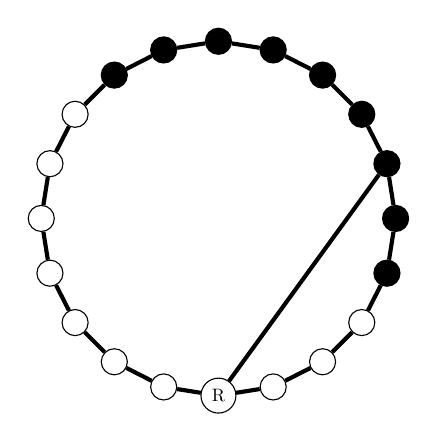
\begin{tikzpicture}[scale=0.25]
\tikzstyle{every node}=[scale=0.5,draw,shape=circle];
\node[scale=2,fill=black] (4) at (-18:9) {};
\node[scale=2,fill=black] (5) at (0:9) {};
\node[scale=2,fill=black] (6) at ( 18:9) {};
\node[scale=2,fill=black] (7) at (2*18:9) {};
\node[scale=2,fill=black] (8) at (3*18:9) {};
\node[scale=2,fill=black] (9) at (4*18:9) {};
\node[scale=2,fill=black] (10) at (5*18:9) {};
\node[scale=2,fill=black] (11) at (6*18:9) {};
\node[scale=2,fill=black] (12) at (7*18:9) {};
\node[scale=2] (13) at (8*18:9) {};
\node[scale=2] (14) at (9*18:9) {};
\node[scale=2] (15) at (10*18:9) {};
\node[scale=2] (16) at ( 11*18:9) {};
\node[scale=2] (17) at (12*18:9) {};
\node[scale=2] (18) at (13*18:9) {};
\node[scale=2] (19) at (14*18:9) {};
\node[scale=1.3] (r) at (15*18:9) {R};
\node[scale=2] (1) at (16*18:9) {};
\node[scale=2] (2) at (17*18:9) {};
\node[scale=2] (3) at (18*18:9) {};
\draw[line width=1.5pt](r)--(1)
(1) -- (2)
(2) -- (3)
(3) -- (4)
(4) -- (5)
(5) -- (6)
(6) -- (7)
(7) -- (8)
(8) -- (9)
(9) -- (10)
(10) -- (11)
(11) -- (12)
(12) -- (13)
(13) -- (14)
(14) -- (15)
(15) -- (16)
(16) -- (17)
(17) -- (18)
(18) -- (19)
(19) -- (r)
(r) -- (6);
\end{tikzpicture}
\caption{ Illustration des nœuds aléatoires (nœuds noires) qui devient plus proche du nœud arbitraire $R$, et nœuds réguliers (nœuds blanches) qui restent dans leurs distance initial par rapport au même nœud arbitraire $R$, le réseau est de taille $n=20$, $k=1$ et un seul raccourci.}

\label{r-al}
\end{figure}
\begin{itemize}
\item[$\blacksquare$]  \`{A} travers $1$ raccourci:\\
Soit $\pi^1(i)$ la probabilité qu'un nœud ne change pas sa distance régulière $j$ vers
la $i^{\text{ème}}$ distance ($i<j$) à travers un seul raccourci:
\begin{eqnarray}\nonumber
	\pi^1(1)&=&(1-q), \\\nonumber
	\pi^1(2)&=&(1-q)^4,\\\nonumber
	\pi^1(3)&=&(1-q)^{4\cdot2},\\\nonumber
	\vdots\\
	\pi^1(i)&=&(1-q)^{4(i-1)}.
	\label{pi1}
	\end{eqnarray}
	Il faut signalé que l'expression $\pi^1(i)=(1-q)^{4(i-1)}$ est une approximation de champs moyenne qu'est vrai pour la plupart des cas et qui représente la valeur minimale de cette probabilité, car les nombres des possibilités
	$4,4\times2,...,4\times(i-1)$ sont les valeurs maximales, mais à cause des interférences entres elles, le nombre de possibilités peut être moindre, la m\^{e}me remarque pour tous les cas 
	suivants, on prend toujours le nombre maximum de possibilité, d'où nos équations sont des approximations de champs moyenne et ne sont pas des expressions 
	mathématiques exactes, certes comme tous les systèmes de très grand nombre de constituants, il suffit de faire la bonne 
	approximation au niveau microscopique, c'est-à-dire local, pour trouver la description parfaite des grandeurs macroscopique de système, ce que nous
	avons exactement fait.\\
	De l'Eq.~\ref{pi1} la probabilité $P^1_r(j)$ qu'un nœud ne change pas sa distance régulière $j$ à travers un seul raccourci est:
	\begin{eqnarray}\nonumber
	P_r^1(j)&=&\pi^1(1)\pi^1(2)...\pi^1(j-1)\\\nonumber
	&=& (1-q)(1-q)^4(1-q)^{4\cdot2}...(1-q)^{4(j-2)}\\\nonumber
	&=&(1-q)^{1+4+4\cdot2+4\cdot3...4(j-2)}\\\nonumber
	&=&(1-q)^{1+4\sum_{i=1}^{j-1}(i-1)}.
	\end{eqnarray}
	On doit signaler qu'on peut négliger le cas $\pi^i(i)=(1-q)^{i}(\acute{n}-2i)^{i-1}$,  dans le cas d'un raccourci et dans tous les cas suivants sans aucun problème, alors $P_r^1(j)$ sera écrite:
	$$P_r^1(j)=(1-q)^{4\sum_{i=1}^{j-1}(i-1)}$$
	
\item[$\blacksquare$]  \`{A} travers $2$ raccourcis: \\
La probabilité qu'un nœud ne change pas sa distance régulière $j$ vers la $i^{\text{ème}}$ distance ($i<j$) à travers deux raccourcis, dans
le cas où le nœud arbitraire lié directement par un raccourci avec un nœud intermédiaire $z$ qui est à une distance $i-1$ du
nœud $j$ à travers aussi un seul raccourci, est $(1-q^2)^{4(i-2)}$. On considère que cette probabilité est la m\^{e}me
pour les autres possibilités d'arrangements de deux  raccourcis autour le nœud intermédiaire.\\ Le nombre
possible des arrangements de ces deux raccourcis autour de nœud intermédiaire $z$ pour lequel la distance entre $j$ et le nœud arbitraire sera toujours $i$ est\footnote{Par exemple dans le cas où $i=4$, on a $3$ des arrangements possibles pour que la distance entre le nœud $j$ et le nombre arbitraire est $4$:\\ le $1^{\text{ère}}$: la distance entre le nœud arbitraire et le nœud intermédier $z$ est $1$ et entre $z$ et le nœud $j$ est $3$.\\ le $2^{\text{ème}}$: la distance entre le nœud arbitraire et le nœud intermédier $z$ est $2$ et entre $z$ et le nœud $j$ est également $2$.\\ le $3^{\text{ème}}$: la distance entre le nœud arbitraire et le nœud intermédier $z$ est $3$ et entre $z$ et le nœud $j$ est $1$.}  $(i-1)$.\\
En outre le nombre maximal possible des positions de $z$ sur le réseau pour que $i<j$ est
$\acute{n}-2i$, alors la probabilité qu'un nœud ne change pas sa distance régulière $j$ vers
la $i^{\text{ème}}$ distance ($i<j$) à travers deux raccourcis est
\begin{eqnarray}
	\pi^2(i)=(1-q^2)^{4(i-1)(i-2)(\acute{n}-2i)},\nonumber
\end{eqnarray}
d'où
\begin{eqnarray}
	P_r^2(j)&=&\pi^2(1)\pi^2(2)...\pi^2(j-1)\\\nonumber
	&=& (1-q^2)^{4\sum_{i=1}^{i=j-1}((i-1)(i-2)(\acute{n}-2i))},
\end{eqnarray}
comme nous avons déjà signalé le terme $\pi^i(i)$ est négligeable, ici est $\pi^2(2)$.\\
	
\item[$\blacksquare$]  \`{A} travers $3$ raccourcis:\\
	Dans ce cas on a deux nœuds intermédiaires $z$ et $\acute{z}$ sous la condition que entre deux nœuds intérimaires il y a un seul raccourci.
	La probabilité qu'un nœud ne change pas sa distance $j$ vers la $i^{\text{ème}}$ distance à travers $3$ raccourcis pour le cas où le
	nœud arbitraire lié directement par un raccourci avec $z$ qui lié aussi directement par un raccourci avec $\acute{z}$ et ce 
	dernière à une distance de $i-2$ au nœud $j$ à travers aussi un seul raccourci, est $(1-q^3)^{4(i-3)}$. On considère que cette probabilité est la m\^{e}me
	pour les autres possibilités d'arrangements de trois raccourcis autour les deux nœuds intermédiaires.\\
	Le nombre possible des
	arrangements de ces trois raccourcis autour des nœuds intérimaires $z$ et $\acute{z}$ pour que la distance entre $j$ et le	nœud arbitraire est toujours $i$ est $C_2^{i-1}=\frac{(i-1)(i-2)}{2!}$.\\
	 En outre le nombre maximal possible des positions de $z$ et
	$\acute{z}$ sur le réseau pour $i<j$ est approximativement $(\acute{n}-2i)^2$.\\
	
	Alors on obtient que $\pi^3(i)=(1-q^3)^{4\frac{(i-1)(i-2)}{2!}(i-3)(\acute{n}-2i)^2}\nonumber$ d'où
	\begin{eqnarray}
	P_r^3(j)&=&\pi^3(1)\pi^3(2)...\pi^3(j-1)\\\nonumber
	&=& (1-q^3)^{4\sum_{i=1}^{i=j-1}(\frac{(i-1)(i-2)}{2!}(i-3)(\acute{n}-2i)^2)}.
	\end{eqnarray}
	
\item[$\blacksquare$] \`{A} travers $4$ raccourcis:\\
Dans ce cas on a trois nœuds intermédiaires $z$,$z'$ et $z''$, toujours sous la condition  qu'il y a un seul raccourci entre chaque deux nœuds
intérimaires. La probabilité qu'un nœud ne change pas sa distance $j$ vers la $i^{\text{ème}}$ distance à travers $4$ raccourcis pour 
le cas où le nœud arbitraire lié directement par un raccourci avec $z$ et celui-ci lié également directement par un raccourci 
avec $z'$ qui est de sa part lié directement par un raccourci avec le nœud $z''$  et ce dernier à une distance de $i-3$ au
nœud $j$ à travers aussi un seul raccourci est $(1-q^4)^{4(i-4)}$.
On considère comme les cas précédent que cette probabilité est la m\^{e}me
pour les autres possibilités d'arrangements de quatre raccourcis autour les trois nœuds intermédiaires.\\ Le nombre possible des arrangements de ces trois raccourcis
autour des nœuds intérimaires $z$,$z'$ et $z''$ pour que la distance entre $j$ et le nœud  arbitraire est $i$ est
$C_3^{i-1}=\frac{(i-1)(i-2)(i-3)}{3!}$.\\ En outre le nombre maximal possible  des positions de $z$,$z'$ et $z''$ sur le réseau pour $i<j$ est  approximativement
$(\acute{n}-2i)^3$.
Alors on obtient
\begin{eqnarray}
	\pi^4(i)=(1-q^4)^{4\frac{(i-1)(i-2)(i-3)}{3!}(i-4)(\acute{n}-2i)^3},\nonumber
	\end{eqnarray}
	d'où
	\begin{eqnarray}
	P_r^4(j)&=&\pi^4(1)\pi^4(2)...\pi^4(j-1)\\\nonumber
	&=& (1-q^4)^{4\sum_{i=1}^{i=j-1}(\frac{(i-1)(i-2)(i-3)}{3!}(i-4)(\acute{n}-2i)^3)}.
	\end{eqnarray}
	
\item[$\blacksquare$] \`{A} travers $m$ raccourcis:\\
Par la m\^{e}me méthode, si on suppose qu'il  y a $(m-1)$ nœuds intermédiaires, on va obtenir l'expression générale de la probabilité qu'un nœud ne change pas sa distance $j$ vers la $i^{\text{ème}}$ distance à travers $m$ raccourcis sous la forme 
\begin{eqnarray}
	\pi^m(i)=(1-q^m)^{4\frac{(i-1)(i-2)\ldots(i-m)}{(m-1)!}(\acute{n}-2i)^{(m-1)}},\nonumber
\end{eqnarray}
alors la probabilité qu'un nœud ne change pas sa distance régulière $j$ à travers $m$ raccourcis est
\begin{eqnarray}
	P_r^m(j)&=&\pi^m(1)\pi^m(2)...\pi^m(j-1)\\\nonumber
	&=& (1-q^m)^{4\sum_{i=1}^{j-1}(\frac{(i-1)(i-2)\ldots(i-m)}{(m-1)!}(\acute{n}-2i)^{m-1})},
	\end{eqnarray}
sachant que $q<1$ on peut écrire 
\begin{eqnarray}
P_r^m(j)=e^{-4q^m\sum_{i=1}^{j-1}(\frac{(i-1)(i-2)\ldots(i-m)}{(m-1)!}(\acute{n}-2i)^{m-1})}.
\end{eqnarray}
\end{itemize}

Alors la probabilité $P_r(j)$ qu'un nœud ne change pas sa distance régulière $j$ vers la $i^{\text{ème}}$ distance par n'importe 
quel nombre des raccourcis est
\begin{eqnarray}
P_r(j)&=&P^1_r(j)P^2_r(j)P^4_r(j)\ldots P^m_r(j)\\\nonumber
&=&e^{-4q\sum_{i=1}^{j-1}(i-1)B(i)}, 
\end{eqnarray}
avec $B(i)=\big(1+[q(i-2)(\acute{n}-2i)]+[q^2\frac{(i-2)(i-3)}{2!}(\acute{n}-2i)^{2}]+\ldots+[q^{m-1}\frac{(i-2)\ldots
	(i-m)}{(m-1)!}(\acute{n}-2i)^{m-1}]+\ldots+[q^{i-2}(\acute{n}-2i)^{i-2}]\big)$, les termes de cette expression lient respectivement
au probabilité que le nœud $j$ ne change pas sa distance vers le $i^{\text{ème}}$ distance par $2,3,4,...,i-1$ raccourcis, le cas de $i$ 
raccourcis est négligé comme nous avons déjà dit. D'une autre coté on voit que $B(i)$ peut s'écrire sous la formule du Bin\^{o}me
\begin{eqnarray}\nonumber
B(i)&=&\big(1+[q(i-2)(\acute{n}-2i)]+[q^2\frac{(i-2)(i-3)}{2!}(\acute{n}-2i)^{2}]+\ldots+[q^{i-2}(\acute{n}-2i)^{i-2}]\big)\\\nonumber
&=&\sum_{j=1}^{i-2}C_j^{i-2}[q(\acute{n}-2i)]^j1^{i-2-j}\\\nonumber
&=&(q(\acute{n}-2i)+1)^{i-2}.
\end{eqnarray}

\begin{figure}[h!]
	\centering 
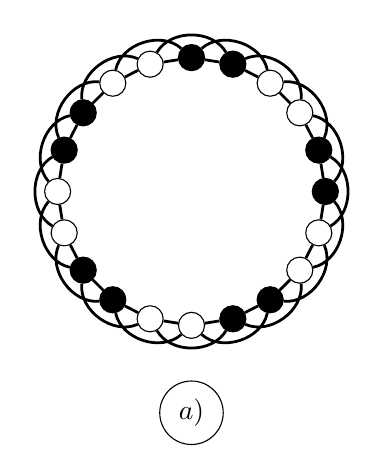
\begin{tikzpicture}[scale=0.2]
\draw (0,-12) node[scale=2,below]{$a)$} ;
\tikzstyle{every node}=[scale=0.5,draw,shape=circle];
\node[scale=2]  (4) at (-18:8.5) {};
\node[scale=2,fill=black] (5) at (0:8.5) {};
\node[scale=2,fill=black] (6) at ( 18:8.5) {};
\node[scale=2] (7) at (2*18:8.5) {};
\node[scale=2] (8) at (3*18:8.5) {};
\node[scale=2,fill=black] (9) at (4*18:8.5) {};
\node[scale=2,fill=black] (10) at (5*18:8.5) {};
\node[scale=2] (11) at (6*18:8.5) {};
\node[scale=2] (12) at (7*18:8.5) {};
\node[scale=2,fill=black] (13) at (8*18:8.5) {};
\node[scale=2,fill=black] (14) at (9*18:8.5) {};
\node[scale=2] (15) at (10*18:8.5) {};
\node[scale=2] (16) at ( 11*18:8.5) {};
\node[scale=2,fill=black] (17) at (12*18:8.5) {};
\node[scale=2,fill=black] (18) at (13*18:8.5) {};
\node[scale=2] (19) at (14*18:8.5) {};
\node[scale=2] (r) at (15*18:8.5) {};
\node[scale=2,fill=black] (1) at (16*18:8.5) {};
\node[scale=2,fill=black] (2) at (17*18:8.5) {};
\node[scale=2] (3) at (18*18:8.5) {};
\draw[line width=1pt](r)--(1)
(1) -- (2)
(2) -- (3)
(3) -- (4)
(4) -- (5)
(5) -- (6)
(6) -- (7)
(7) -- (8)
(8) -- (9)
(9) -- (10)
(10) -- (11)
(11) -- (12)
(12) -- (13)
(13) -- (14)
(14) -- (15)
(15) -- (16)
(16) -- (17)
(17) -- (18)
(18) -- (19)
(19) -- (r);
\draw[line width=1pt] (r) to [bend right=60] (2) 
(2)to [bend right=60](4)
(4)to [bend right=60](6)
(6)to [bend right=60](8)
(8)to [bend right=60](10)
(10)to [bend right=60](12)
(12)to [bend right=60](14)
(14)to [bend right=60](16)
(16)to [bend right=60](18)
(18)to [bend right=60](r)

(1)to [bend right=60](3)
(3)to [bend right=60](5)
(5)to [bend right=60](7)
(7)to [bend right=60](9)
(9)to [bend right=60](11)
(11)to [bend right=60](13)
(13)to [bend right=60](15)
(15)to [bend right=60](17)
(17)to [bend right=60](19)
(19)to [bend right=60](1);
\end{tikzpicture}
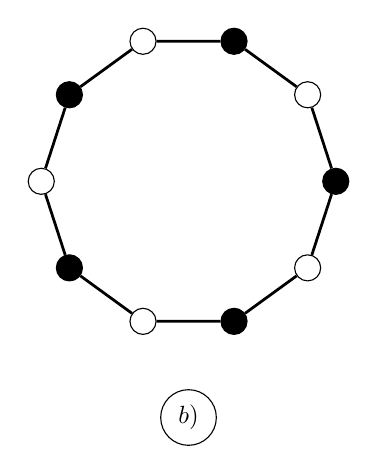
\begin{tikzpicture}[scale=0.22]
\draw (0,-12) node[scale=1.8,below]{$b)$} ;
\tikzstyle{every node}=[scale=0.5,draw,shape=circle];
\node (4)[scale=2] at (-36:8.5) {};
\node (5)[scale=2,fill=black]  at (0:8.5) {};
\node (6)[scale=2] at ( 36:8.5) {};
\node (7)[scale=2,fill=black]  at (2*36:8.5) {};
\node (8)[scale=2] at (3*36:8.5) {};
\node (9)[scale=2,fill=black]  at (4*36:8.5) {};
\node (r)[scale=2] at (15*36:8.5) {};
\node[scale=2,fill=black] (1) at (16*36:8.5) {};
\node (2)[scale=2] at (17*36:8.5) {};
\node[scale=2,fill=black]  (3) at (18*36:8.5) {};
\draw[line width=1pt](r)--(1)
(1) -- (2)
(2) -- (3)
(3) -- (4)
(4) -- (5)
(5) -- (6)
(6) -- (7)
(7) -- (8)
(8) -- (9)
(9) -- (r);
%\node[scale=3,text centered] at (0,-12) {b)};
\end{tikzpicture}
\caption{La transformation GR d'un réseau (a) de $n=20$ et $k=2$ vers un réseau (b) de $\acute{n}=10$ et $\acute{k}=1$.}
\label{RG}
\end{figure}
Alors la probabilité qu'un nœud ne change pas sa distance $j$ est: 
\begin{eqnarray}
\label{pr}
P_r(j)&=& e^{-4q\sum_{i=1}^{j-1}(i-1)(q(\acute{n}-2i)+1)^{i-2}}\\\nonumber
&=&e^{-4q\int_{i=1}^{j-1}(i-1)(q(\acute{n}-2i)+1)^{i-2}di}.
\end{eqnarray}

En outre la probabilité $P_{al}(j)$ qu'un nœud change sa distance régulière vers la  $j^{\text{ème}}$ égale le produit de la probabilité que ce nœud ne change pas sa distance vers une autre inférieur à  $j$, $P_r(j-1)$, et la probabilité que le nœud change sa distance vers la $j^{\text{ème}}$ distance,$1-\pi(j)$,
\begin{eqnarray}\nonumber
P_{al}(j)&=&P_r(j-1)(1-\pi(j))\\\nonumber
&=&P_r(j-1)-\pi(j)P_r(j-1)\\\nonumber
&=&P_r(j-1)-P_r(j)\\\nonumber
&=&-\frac{\partial P_r(j)}{\partial j}\\
&=&4q(j-2)(q(\acute{n}-2(j-1)-1))+1)^{j-3}P_r(j),
\end{eqnarray}
pour simplifier les calculs on peut prendre sans aucun souci\footnote{Cette approximation signifie une augmentation de l'erreur de l'ordre $\frac{1}{\ell}$, cependant $\ell$ tend vers l'infini lorsque $n$ est très large, alors cette approximation ne pose aucun problème.} que dans l'équation précédent $j-1=j$, d'où on obtient
\begin{eqnarray}
P_{al}(j)=4q(j-1)(q(\acute{n}-2j-1))+1)^{j-2}P_r(j).
\label{pal}
\end{eqnarray}
Le nombre des nœuds dans la couche $n_{j}^r$ est $P_r(j)$ multiplié par $2$, car initialement dans chaque couche on a  deux nœuds réguliers
\begin{eqnarray}
n_{j}^r=2P_r(j),
\label{cr}
\end{eqnarray}
et le nombre des nœuds dans le couche aléatoire $n_{j}^{al}$ est $P_{al}(j)$ multiplié par le nombre des nœuds qui ont une distance plus grande que $j$
\begin{eqnarray}
n_{j}^{al}=(\acute{n}-2j)P_{al}(j),
\label{cal}
\end{eqnarray}
d'où la $j^{\text{ème}}$ couche est
\begin{eqnarray}
n_j&=&n_{j}^{r}+n_{j}^{al}\\\nonumber
&=&2P_r(j)+(\acute{n}-2j)P_{al}(j)\\\nonumber
&=&2P_r(j)+(\acute{n}-2j)P_r(j-1)-(\acute{n}-2j)P_r(j)\\\nonumber
&=&(\acute{n}-2j)P_r(j-1)-(\acute{n}-2(j+1))P_r(j)\\\nonumber
&=&v(j-1)-v(j) \quad \quad  \text{avec:} \quad v(j)=(\acute{n}-2(j+1))P_r(j).
\nonumber
\label{c}
\end{eqnarray}
Maintenant on va calculer la somme des nœuds de couches-régulières $S'_r$ et la somme des nœuds de couches-aléatoires $S'_{al}$ afin de les utiliser dans le calcul de PCC. De Eq.~\ref{pr} et Eq.~\ref{cr} on obtient

\begin{eqnarray}
S'_r &=&n_{1}^{r}+\sum^{\frac{\acute{n}}{2}}_2n_{i}^{r}\\\nonumber
&=&n_{1}^{r}+\int^{\frac{\acute{n}}{2}}_2n_{i}^{r}di\\\nonumber
&=&n_{1}^{r}+2\int^{\frac{\acute{n}}{2}}_2e^{-4q\int_{j=1}^{i-1}(j-1)(q(\acute{n}-2j)+1)^{j-2}dj}di,\nonumber
\end{eqnarray}
l'intégrale $\int^{\frac{\acute{n}}{2}}_2e^{-4q\int_{j=1}^{i-1}(j-1)(q(\acute{n}-2j)+1)^{j-2}dj}di$, n'a aucune solution disponible, pour cette raison, on est obligé d'utiliser une approximation en tenant compte seulement les chemins à travers un seul raccourci et on néglige les autres.\\
L'approximation s'avère vrai dans la première région où le nombre des raccourcis est très faible, par contre dans
la seconde région où le nombre des raccourcis est grand n'est pas vrai, néanmoins la fraction des nœuds de réseau régulier dans la seconde région est très petit, pour cette raison cette approximation est valable pour les deux régions. Alors on prend que 
$\int^{\frac{\acute{n}}{2}}_2e^{-4q\int_{j=1}^{i-1}(j-1)(q(\acute{n}-2j)+1)^{j-2}dj}di\approx\int^{\frac{\acute{n}}{2}}_2e^{-4q\int_{j=1}^{i-1}(j-1)dj}di$.
Pour $\acute{n}\gg 1$ on peut prendre que $ \int^{\frac{\acute{n}}{2}}_2e^{-4q\int_{j=1}^{i-1}(j-1)dj}di\approx\int^{\frac{\acute{n}}{2}}_2e^{-4q\int_{j=1}^{i}jdj}di$,
d'où:
\begin{eqnarray}
\label{sr}
S'_r &\approx&n_{1}^{r}+2\int^{\frac{\acute{n}}{2}}_2e^{-4q\int_{j=1}^{i}jdj}di\\\nonumber
&\approx&n_{1}^{r}+2\int^{\frac{\acute{n}}{2}}_2e^{-2qi^2}di\\\nonumber
&\approx&2+2\Big[\frac{\sqrt{\frac{\pi}{2}}erf(\sqrt{2q}i)}{2\sqrt{q}}\Big]^{\frac{\acute{n}}{2}}_2 \hspace{1cm}
\textrm{avec }  n_{1}^{r}=2 \\\nonumber
&\approx&2+ 2\sqrt{\frac{\pi}{8q}}\Big[erf(\sqrt{2q}\frac{\acute{n}}{2})-erf(2\sqrt{2q})\Big], \nonumber
\end{eqnarray}
pour $q\ll 1$ on a $erf(2\sqrt{2q})=\dfrac{2}{\sqrt{\pi}}2\sqrt{2q}$ alors on obtient

\begin{eqnarray}
S'_r&\approx&2+ 2\sqrt{\frac{\pi}{8q}}\Big[erf(\sqrt{2q}\frac{\acute{n}}{2})-\dfrac{2}{\sqrt{\pi}}2\sqrt{2q}\Big] \\\nonumber
&\approx& 2+2\sqrt{\frac{\pi}{8q}}erf(\sqrt{\frac{q\acute{n}^2}{2}})-4  \\\nonumber
&\approx& \acute{n}\Big(\sqrt{\frac{\pi}{2q\acute{n}^2}}erf(\sqrt{\frac{q\acute{n}^2}{2}})-\frac{2}{n'}\Big)  \\\nonumber
&\approx& \acute{n}\sqrt{\frac{\pi}{2q\acute{n}^2}}erf(\sqrt{\frac{q\acute{n}^2}{2}}).\nonumber
\end{eqnarray}
On sait que $q=\frac{2k^3\phi}{n}$ et $\acute{n}=\frac{n}{k}$ alors $\frac{q\acute{n}^2}{2}=kn\phi$ qui est le
nombre moyen des raccourcis dans le réseau, d'où  la somme des nœuds réguliers s'écrit aussi comme une
fonction universelle, sous la forme
\begin{eqnarray}
S'_r=\frac{n}{k}(1-h(kn\phi)),
\end{eqnarray}
avec $h(x)=1-\sqrt{\frac{\pi}{4x}}erf(\sqrt{x})$\\

En outre la somme des nœuds aléatoires est la soustraction du nombre de nœuds et la somme des nœuds
réguliers 
%, en plus on soustraire $1$ car le noeud numéro $\frac{n}{2}$ a compté deux fois dans l'expression de $S_r$,
%ce n'est pas $1$ exactement qu'il faut soustraire ... mais le compte de ce noeud est important pour le nombre des raccorsis
%trés inférieur à $1$ où les raccorci n'a pas encore d'inflience, 
\begin{eqnarray}
S'_{al}&\approx&\acute{n}-S'_r\\\nonumber
&\approx& \acute{n}-\acute{n}\sqrt{\frac{\pi}{2q\acute{n}^2}}erf(\sqrt{\frac{q\acute{n}^2}{2}})  \\\nonumber
&\approx& \acute{n}\Big(1-\sqrt{\frac{\pi}{2q\acute{n}^2}}erf(\sqrt{\frac{q\acute{n}^2}{2}})\Big)  \\\nonumber
&\approx& \frac{n}{k}h(kn\phi).\nonumber
\end{eqnarray}
\begin{figure}[h!]
	\centering
	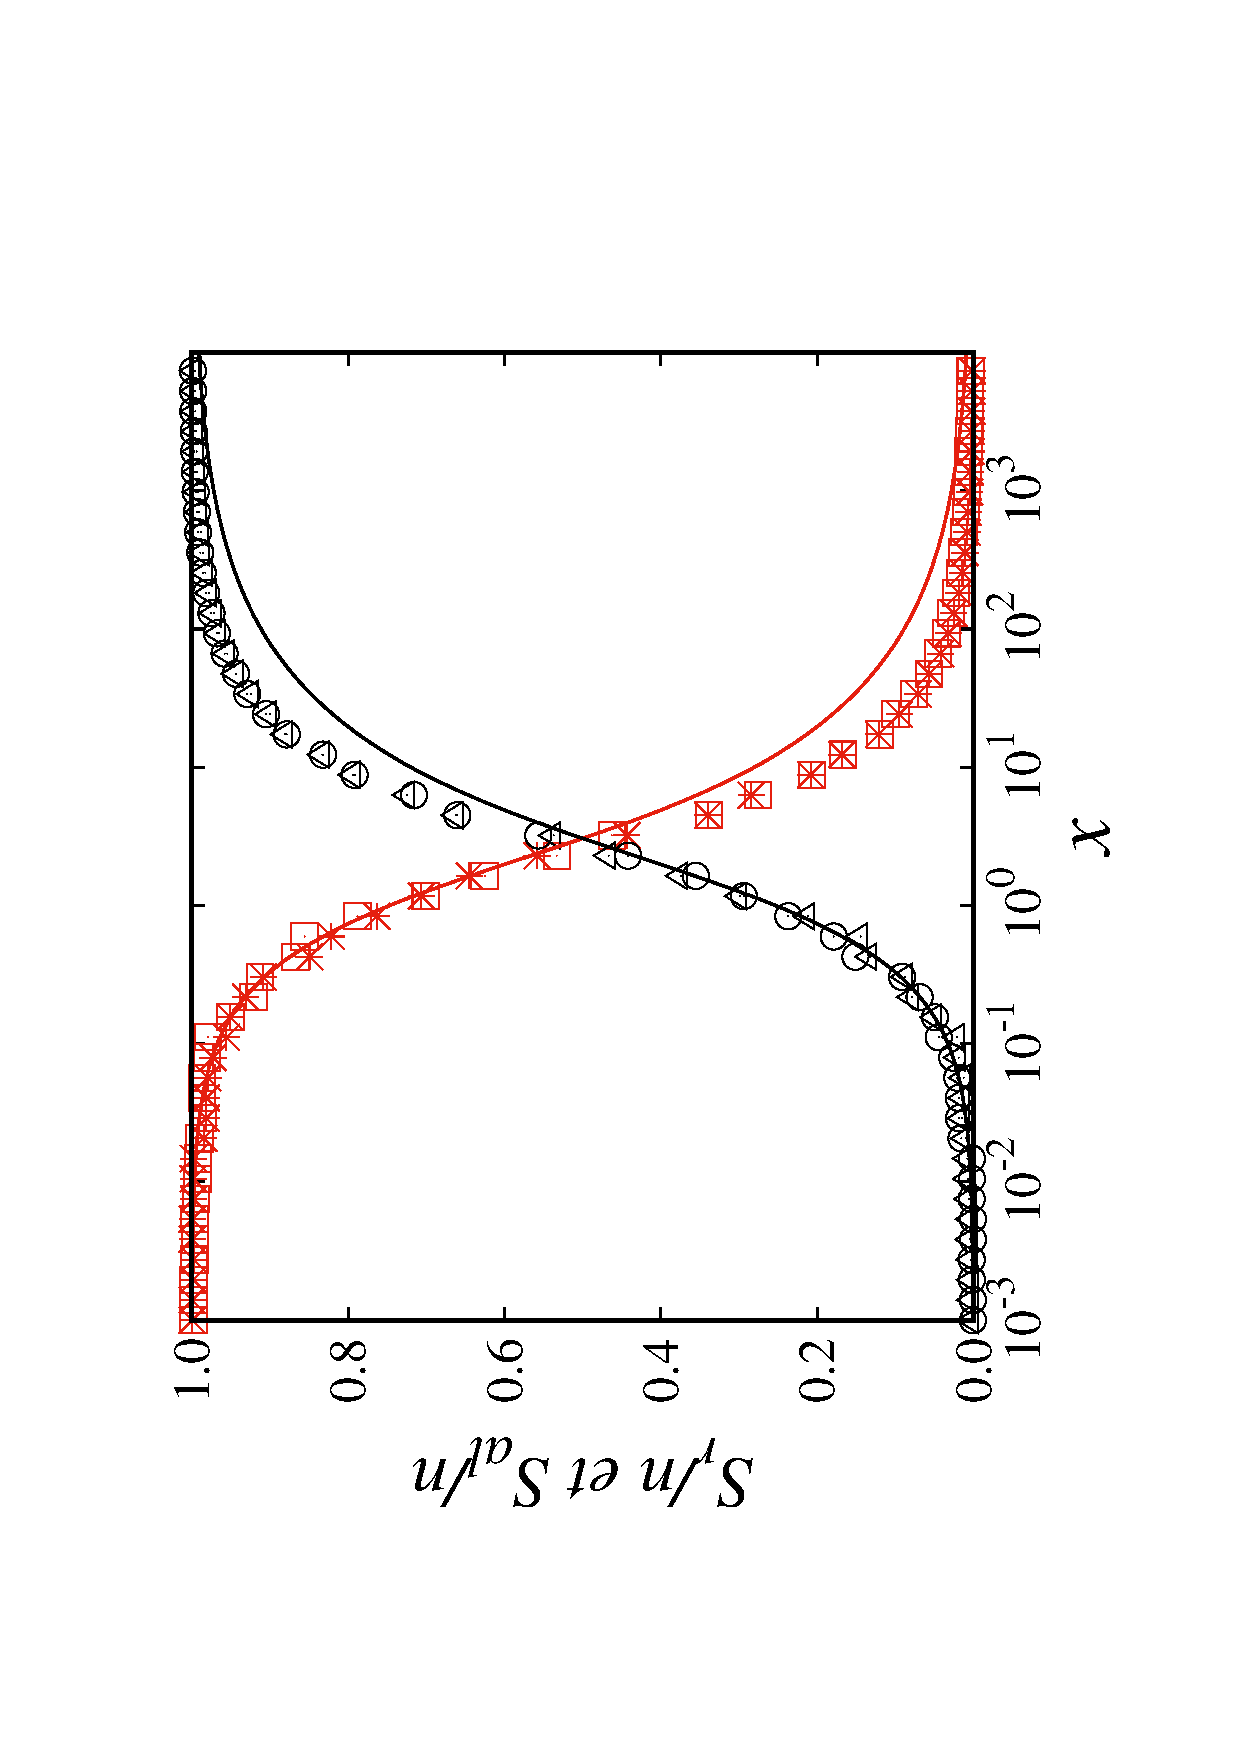
\includegraphics[scale=0.5,angle=-90]{./figures/fig-s}
	\caption{Fraction des nœuds aléatoires $S_{al}/n$ 
		(noir) et des nœuds réguliers $S_{r}/n$ (rouge)  en fonction de nombre des raccourcis $x$. Les lignes représentent les fonction $h(x)$  (noir) et $1-h(x)$ (rouge). Les symboles représentent les simulations numériques d'un réseau de taille $n=10^4$, avec
		$k=1$ (étoile et cercle) et $k=5$ (carré et triangle). Chaque simulation est moyennée à $200$ réalisations.}
	\label{S}
\end{figure}

Si on prend en considération la transformation de GR  qu'on a déjà utilisé dans nos calculs, les valeurs de $S'_{r}$ et $S'_{al}$ représentent en réalité le nombre des groupes $k$ de nœuds,
alors pour trouver le nombre réel des nœuds dans le réseau, il suffit de multiplier $S'_{r}$ et $S'_{al}$  par $k$
, car dans chaque groupe on a $k$ nœuds, d'où le nombre des nœuds réguliers est $S_r=n(1-h(kn\phi))$ et le nombre de nœuds 
aléatoires est $S_{al}=n h(kn\phi)$.
Sachant que la fonction $h(x)$ peut être considéré comme un paramètre d'ordre et selon son expression, on peut conclure qu'il n'y a pas une transition de phase dans ce modèle mais un phénomène de croisement qui commence depuis $x=0$. L'existence d'un tel paramètre d'ordre dans le modèle de NW est déjà une chose très importante, car il n'est pas toujours facile de le trouve, ainsi l'absence  d'un tel paramètre de ce modèle dans la littérature.  

\subsection{Plus court chemin}
On sait que l'expression du PCC s'écrit  $\ell=\sum_{i=1}^{\frac{\acute{n}}{2}}(i\cdot n_i)$, mais cette somme n'a pas une solution 
directe. Pour cette raison on va dissocier le PCC en deux types, exactement comme le cas des couches, d'où $\ell=\ell_{al}+\ell_r$, avec $\ell_r$ est le PCC du réseau régulier  et $\ell_{al}$ est le PCC du réseau aléatoire.\\
On commence par le PCC de réseau régulier $\ell_r$ qui s'écrit sous la forme 
\begin{equation}
\ell_r=\frac{S'_r}{\acute{n}}\frac{\int_1^{\frac{\acute{n}}{2}}i\cdot n_{i}^{r}di}{a_r},
\end{equation}
avec $a_r=\int_1^{\frac{\acute{n}}{2}}n_{i}^{r}di=S'_r$
est la constante de normalisation, d'où $\ell_r=\int_1^{\frac{\acute{n}}{2}}i\cdot\frac{n_{i}^{r}}{\acute{n}}di$.\\
De Eq.~\ref{pr} et Eq.~\ref{cr} on obtient
\begin{eqnarray}
\ell_r&=&\frac{1}{\acute{n}}\int^{\frac{\acute{n}}{2}}_1 2ie^{-4q\int_{j=1}^{i-1}(j-1)(q(\acute{n}-2j)+1)^{j-2}dj}di,\nonumber
\end{eqnarray}
en utilisant la m\^{e}me approximation précédente de l'Eq.~\ref{sr} on obtient
\begin{eqnarray}
\ell_r &\approx&\frac{1}{\acute{n}}\int_1^{\frac{\acute{n}}{2}}2ie^{-2qi^2}di \\\nonumber
&\approx&\frac{1}{\acute{n}}\frac{e^{-2q}-e^{-\frac{q\acute{n}^2}{2}}}{2q}\\\nonumber
&\approx&\frac{1}{\acute{n}}\frac{1-e^{-\frac{q\acute{n}^2}{2}}}{2q} \quad \quad  \text{car:} \quad q\ll1 \\\nonumber
&\approx&\frac{\acute{n}}{4}\frac{1-e^{-\frac{q\acute{n}^2}{2}}}{\frac{q\acute{n}^2}{2}},\nonumber
\end{eqnarray}
sachant que $\frac{q\acute{n}^2}{2}=nk\phi=x$ et $\acute{n}=\frac{n}{k}$ alors $\ell_r$ peut s'écrire sous la forme universelle suivante
\begin{eqnarray}
\ell_r&\approx&\frac{n}{k}f_r(x) \quad \quad \textrm{avec} \quad f_r(x)=\frac{1-e^{-x}}{4x}.
\label{lr}
\end{eqnarray}

A fin de calculer $\ell_{al}$, nous utilisons la proposition que le PCC est la position de la couche maximale (voir Section.~\ref{pcc}). Dans notre cas ici c'est la position de la couche aléatoire maximale, de point de vue mathématique il suffit de résoudre $\frac{\partial n'_{al}(i)}{di}=0$. Soit $u(i)=4q(i-1)(q(\acute{n}-2i)+1)^{i-2}$, de l'Eq.~\ref{pr} et Eq.~\ref{pal} on obtient que $P_{al}(i)=u(i)e^{-\int_{j=1}^{i-1}u(j)dj}$. D'autre coté, il est évident que $\ell_{al}$ prédomine dans l'expression du PCC si $S_{al}\gg S_r$, alors la dimension de PCC devient négligeable devant la dimension de $\acute{n}$ car le nombre de raccourcis dans le réseau est important, d'où on peut prendre que $\acute{n}-2i\approx \acute{n}$, donc
$u(i)=4q(i-1)(q\acute{n}+1)^{i-2}$. Soit  $y=q\acute{n}$ le paramètre qui représente le degré moyen de raccourcis pour chaque nœud après la transformation de GR, car $q$ est la probabilité pour qu'un pair de nœuds se connecte et $\acute{n}$ est le nombre de nœuds.\\
 De l'Eq.~\ref{cal} et $P_{al}(i)=u(i)e^{-\int_{j=1}^{i-1}u(j)dj}$  on obtient
\begin{eqnarray}
n'_{al}(i)=\acute{n}u(i)e^{-\int_{j=1}^{i-1}u(j)dj},
\end{eqnarray}
donc 
\begin{eqnarray}
\frac{\partial n'_{al}(i)}{\partial i}&=&\acute{n}\frac{\partial u(i)}{\partial i}e^{-\int_{j=1}^{i-1}u(j)dj}+\acute{n}u(i)\frac{\partial e^{-\int_{j=1}^{i-1}u(j)dj}}{\partial i}\\\nonumber
&=&\acute{n}\frac{\partial u(i)}{\partial i}e^{-\int_{j=1}^{i-1}u(j)dj}-\acute{n}u(i)^2e^{-\int_{j=1}^{i-1}u(j)dj},\nonumber
\end{eqnarray}
alors la solution de $\frac{\partial n'_{al}(i)}{\partial i}=0$ est la solution de l'équation suivante
\begin{equation}
\frac{\partial u(i)}{\partial i}-u(i)^2=0.
\label{28}
\end{equation}
On a $\frac{\partial u(i)}{\partial i}=u(i)\big[\frac{1}{i-1}+\ln(y+1)\big]$ et on sait que $ln(y+1)\gg\frac{1}{i-1}$, car $i$ reflet ici la valeur de PCC qui croit avec la taille 
du réseau $\acute{n}$, alors si $\acute{n}$ croit l'expression $\frac{1}{i-1}$ tend vers $0$, par contre $y=2k^2\phi$ ne dépend pas de la taille de réseau, d'où on peut négliger $\frac{1}{i-1}$ devant
$\ln(y+1)$ et  on obtient $\frac{\partial u(i)}{\partial i}=u(i)ln(y+1)$.\\
Alors l'Eq.~\ref{28} devient
\begin{equation}
u(i)=\ln(y+1),
\label{29}
\end{equation}
si on remplace $u(i)$ par son expression $u(i)=4q(i-1)(q\acute{n}+1)^{i-2}=4q(i-1)(y+1)^{i-2}$, on va trouver la solution de l'Eq.~\ref{29} qui nous 
donne la position de la couche-aléatoire maximal $i_{max}$ 
\begin{equation}
i_{max}=\frac{W\big(\frac{\ln(y+1)^2(y+1)}{4q}\big)}{\ln(y+1)}+1,
\end{equation}
avec $W(x)$ est la fonction de Lambert.\\
Alors selon notre proposition, la valeur de $\ell_{al}$ est $i_{max}$ multiplié par la fraction des nœuds aléatoires $\ell_{al}=i_{max}h(x)$, d'où 
\begin{equation}
\ell_{al}=(\frac{W\big(\frac{y+1)^2(y+1)}{4q}\big)}{\ln(y+1)}+1)h(x).
\label{lal}
\end{equation}
\begin{figure}[h!]
	\centering
	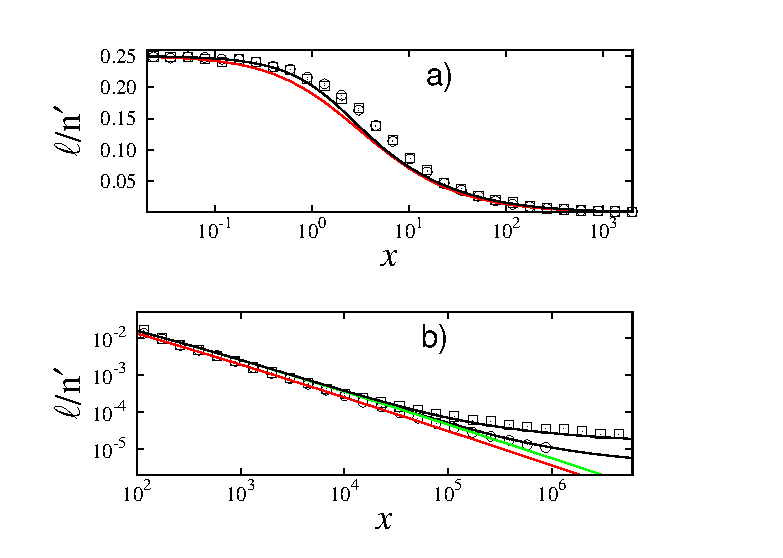
\includegraphics[scale=1.25,angle=0]{./figures/fig-kpn}
	\caption{L'expression universelle $f(x)=\ell/\acute{n}$ en fonction de $x$ pour un réseau de taille $n=10^6$. La formule de Newman et watts Eq.~\ref{eq-ws} (ligne rouge), Eq.~\ref{l2} (ligne vert), Eq.~\ref{l} (ligne noir) et les simulations numériques pour $k=1$ (cercle) et $k=5$ (carré). L'échelle est linéaire-log dans \textbf{a)} et log-log dans \textbf{b)}. Chaque simulation est moyennée à $100$ réalisations.}
	\label{chemin}
\end{figure}

De l'Eq.~\ref{lr} et Eq.~\ref{lal} on obtient l'expression globale de PCC 
\begin{equation}
\ell=\bigg(\frac{W\big(\frac{\ln(y+1)^2(y+1)}{4q}\big)}{ln(y+1)}+1\bigg)h(x)+\acute{n}\frac{1-e^{-x}}{4x}
\label{l}
\end{equation}
pour trouver une expression universelle de $l$ en fonction du nombre des raccourcis $x$, il faut considérer que $y\ll 1$, d'où
\begin{eqnarray}
\ell=\acute{n}f(x) 
\label{l2}
\end{eqnarray}
avec $f(x)=\big(\frac{2W(\frac{x}{2})h(x)+1-e^{-x}}{4x}\big)$ est la nouvelle fonction universelle.\\
De la Fig.~\ref{chemin}, on voit que l'Eq.~\ref{l} est en accord avec les simulations sauf dans l'intervalle
$1<x<20$  où il y a une certaine déviation, on explique cela par la proposition de l'existence des fluctuations élevé dans cette intervalle, car il est évident que lorsque les fluctuations devient importantes l'approximation du champs moyen n'est plus valable,  comme le cas usuel dans tous les systèmes physiques au voisinage des points critiques. On montre notre proposition par les simulations en utilisant le paramètre
d'ordre, $\frac{S_{al}}{n}$.
Soit $\sigma=\frac{\sqrt{\textless \frac{S_{al}}{n}^2\textgreater-\textless \frac{S_{al}}{n}\textgreater^2}}{\textless \frac{S_{al}}{n}\textgreater}$
les fluctuations de $\frac{S_{al}}{n}$ par rapport à sa taille,  en effet selon la Fig.~\ref{fluct} le maximum des fluctuations
est dans l'intervalle $1<x<20$ où l'Eq.~\ref{l} montre une petite déviation.\\

\begin{figure}[h!]
	\centering
	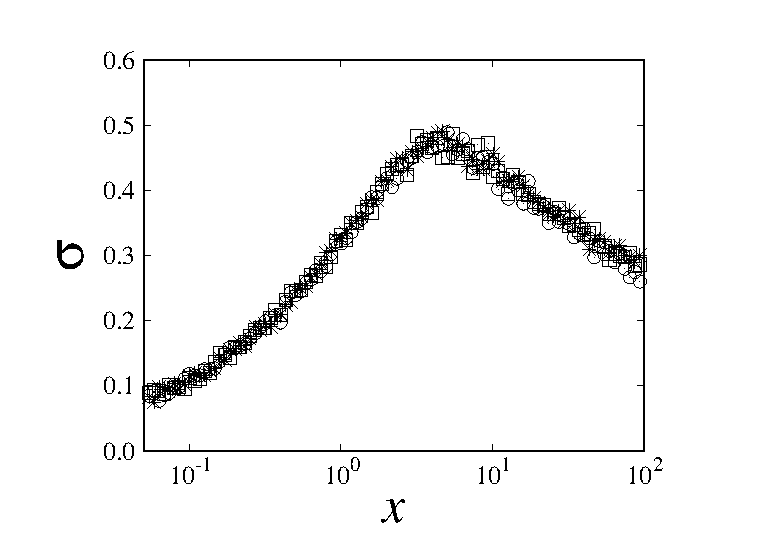
\includegraphics[scale=1,angle=0]{./figures/fig-f}
	\caption{Fluctuation $\sigma$ en fonction de $x$ d'un réseau de taille $n=10^4$  pour différents valeurs de $k$, $k=1$ (étoile), $k=2$ (carré) et $k=5$ (cercle), le nombre de réalisations est $1000$.}
	\label{fluct}
\end{figure}

\section{Émergence spectaculaire vers la propriété petit-monde}
\subsection{Échoué de l'ancien fonction universelle et la saturation des raccourcis}
Selon l'Eq.~\ref{l}, l'expression universel $\ell=\acute{n}f(x)$
n'est plus valable si la condition $y\ll 1$ n'est pas vérifié, qu'on peut aussi montrer par les simulations numériques. Soit $\Delta$ l'écart de $\frac{\ell}{\acute{n}}$ en fonction
de $y$ entre un réseau de $n$, $k$ et $\phi$ donné et d'autres réseaux possédant des valeur aléatoires $n_{al}$, $k_{al}$ 
et $\phi_{al}$ sous la condition que $nk\phi=n_{al}k_{al}\phi_{al}$. L'expression de l'écart de $\frac{\ell}{\acute{n}}$  peut s'écrire  comme
\begin{equation}
\Delta=\frac{\frac{\ell}{\acute{n}}-\frac{\ell_{al}}{\acute{n_{al}}}}{\frac{\ell}{\acute{n}}+\frac{\ell_{al}}{\acute{n_{al}}}}.
\end{equation}

\begin{figure}[h!]
	\centering
	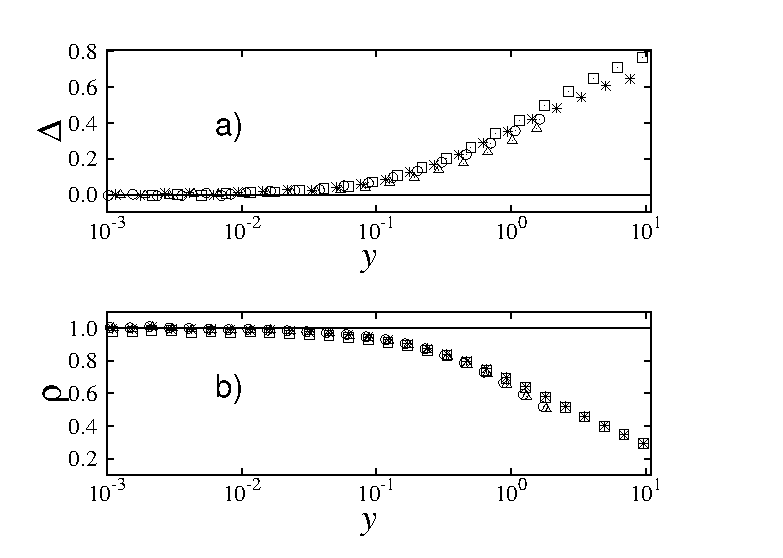
\includegraphics[scale=0.95,angle=0]{./figures/fig3-4}
	\caption{La valeur de $\Delta$ et $\rho$ en fonction de $y$ pour différent valeurs de $n$ et $k$:$n=10^{-3}$ et $k=1$ (triangle), $n=10^{-3}$ et	$k=4$ (carré),$n=10^{-4}$ et $k=1$ (cercle),$n=10^{-4}$ et $k=4$ (étoile). Dans   \textbf{a)} le nombre de réalisations pour chaque simulation est $1000$ et dans \textbf{b)} le nombre de réalisations pour chaque simulation est $5000$.}
	\label{def}
\end{figure}

De la Fig.~\ref{def}.(a) on observe une augmentation remarquable de $\Delta$ lorsque
$y$ n'est pas très inférieur à $1$, par intuition on peut expliquer ce phénomène par le début d'une saturation de raccourcis lorsque $y$ augmente, car après la saturation le réseau change son comportement devant les raccourcis ajoutés. Afin de montrer l'existence d'un changement de comportement vis-à-vis des raccourcis ajoutés, on va simuler numériquement le nombre de raccourcis existe dans le trajet de PCC entre deux nœuds choisi au hasard par rapport au nombre moyen des raccourcis dans le réseau, $\rho$, en fonction de $y$. En effet, selon les Fig.~\ref{def}.(a) et Fig.~\ref{def}.(b), on remarque une saturation de raccourcis qui varie d'une façon similaire avec $\Delta$ en fonction de $y$. Pour $y\ll1$ on voit que $\rho\approx1$, alors presque tous les raccourcis existent dans les trajets de PCC, c'est-à-dire l'impact des raccourcis sur le PCC est maximale, en revanche avec l'augmentation de $y$ le pourcentage des raccourcis existent dans les trajets diminue, c'est-à-dire l'impact des raccourcis sur le PCC se diminue.
On conclu que la saturation des raccourcis ajoutés explique bien la non validité de la fonction universelle $f(x)$ pour  $y\ll1$.\\
 
\subsection{La nouvelle fonction universelle }
La saturation des raccourcis peut signifier que le réseau commence à posséder la propriété petit-monde,
autrement dit le PCC devient de l'ordre de $\ln(n)$, pour confirmer cette proposition on réalise des simulations numériques et on  les compare avec notre équation. En effet, de la Fig.~\ref{fu} on voit que le rapport
$\frac{\ln(n)}{\ell}$ émerge et devient important d'une façon universelle en fonction du même paramètre $y$ avec lequel la saturation émerge. Alors une nouvelle équation universelle $g$ sous la forme $g(y)=\frac{\ln(n)}{\ell}$ apparaît.\\

Maintenant on essaye de formuler l'expression analytique de cette nouvelle équation universelle $g$, de l'Eq.~\ref{l} on peut trouver facilement que dans la limite de grande taille de système on va obtenir que
\begin{eqnarray}
\frac{\ln(n)}{\ell}=\ln(y+1).
\label{kp1}
\end{eqnarray}

\begin{figure}[h!]
	\centering
	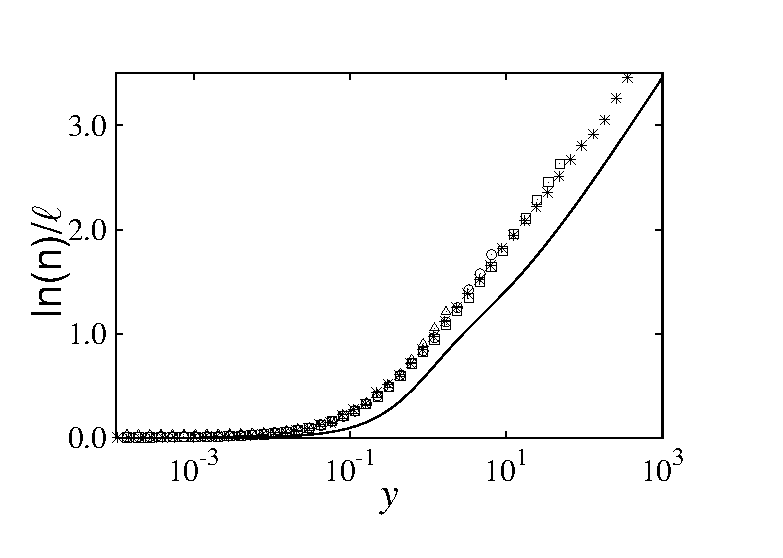
\includegraphics[scale=1,angle=0]{./figures/fig4-4}
	\caption{L'expression universelle de PCC en fonction de $y$, par Eq.\ref{kp2} (ligne continue) et par les simulations numériques pour différents valeurs de $n$ et $k$, $n=10^{-6}$ et $k=20$ (étoile), $n=10^{-5}$ et $k=5$ (carré), $n=10^{-4}$ et $k=2$ (cercle),$n=10^{-3}$ et $k=1$ (triangle), nombre de réalisations pour chaque simulations est $100$. En \textbf{a)} l' échelle est linéaire-log et en \textbf{b)} l'échelle est log-log.}
	\label{fu}
\end{figure}

Il est évident que l'Eq.~\ref{kp1} n'est pas une expression exacte à cause de la transformation de GR que nous avons utilisé au début lorsque nous avons supposé que chaque $k$ voisins, on le dénommé ici \textsf{amas}, est comme  un seul nœud.\\
Sur le trajet de PCC entre deux amas quelconques dans le réseau on trouve des liens ordinaires et des raccourcis, dans le cas où il y a deux raccourcis successifs sur le trajet, c'est-à-dire on a deux raccourcis liant au m\^{e}me \textsf{amas}, la probabilité que les deux raccourcis liant au m\^{e}me nœuds dans cette amas est $\frac{1}{k}$ et la probabilité que les deux raccourcis ne lient pas au m\^{e}me nœud, c'est-à-dire on aura un lien en plus, est  $1-\frac{1}{k}$, autrement dit chaque fois on a deux raccourcis successifs il y a une probabilité de $1-\frac{1}{k}$ que le PCC augment par $1$.\\
D'autre part, le nombre des liens réguliers qui lient entre les \textsf{amas} est toujours
$\acute{n}$ et le nombre des raccourcis entre les \textsf{amas} est $\frac{q\acute{n}(\acute{n}-1)}{2}\approx\frac{q\acute{n}^2}{2}$, 
$q$ est la probabilité qu'un pair d'amas se connecte et $\frac{\acute{n}(\acute{n}-1)}{2}$ est le nombre des pairs possibles. Alors la fraction des raccourcis par rapport au nombre totale des liens est $\frac{q\acute{n}}{2+q\acute{n}}=\frac{y}{2+y}$, d'où la probabilité d'obtenir deux raccourcis liant au m\^{e}me \textsf{amas} dans le trajet entre deux nœuds quelconque est $(\frac{y}{2+y})^2$. Par conséquent la probabilité pour que la valeur de PCC sera doublé est $(\frac{y}{2+y})^2(1-\frac{1}{k})$, où $(\frac{y}{2+y})^2$ est la probabilité d'avoir deux 
raccourcis liant au m\^{e}me \textsf{amas}, et $(1-\frac{1}{k})$ est la probabilité que ces deux amas seront liant à deux nœuds différent. La probabilité que le PCC restera sans aucun changement est $(1-(\frac{y}{2+y})^2)+\frac{1}{k}(\frac{y}{2+y})^2$, le première terme représente la probabilité que deux raccourcis n'est pas liant au m\^{e}me \textsf{amas} et le deuxième représente la probabilité 
que deux raccourcis liant au m\^{e}me \textsf{amas} et au m\^{e}me nœud $\frac{1}{k}(\frac{y}{2+y})^2$, d'où l'Eq.\ref{kp1} devient
\begin{eqnarray}
\frac{\ln(n)}{l}=\frac{\ln(y+1)}{\frac{1}{k}(\frac{y}{2+y})^2+(1-(\frac{y}{2+y})^2)+2(1-\frac{1}{k})(\frac{y}{2+y})^2}
\end{eqnarray}
pour $k\gg1$ on obtient que
\begin{eqnarray}
\frac{\ln(n)}{\ell}=\frac{\ln(y+1)}{\big(1+(\frac{y}{2+y})^2\big)}
\label{kp2}
\end{eqnarray}
Cette fonction montre un certain écart par rapport aux résultats numériques, car dans notre calcul on n'a pas pris en compte tous les cas possibles des raccourcis entre les \textsf{amas} mais on a fait juste une approximation de champs moyen. Cependant notre
expression de $g(y)=\frac{\ln(y+1)}{\big(1+(\frac{y}{2+y})^2\big)}$ nous donne l'allure de la variation de la fonction universelle, qui varie d'une façon logarithmique.\\
Le fait qu'on a réussi à contrôler le nombre des raccourcis ajoutés pour atteindre la phase petit-monde dans le modèle de NW est une chose très importante et une contribution qui va enrichir tellement l'utilité de ce modèle. La difficulté qu'a empêché à répondre à ce problème  au cours des vingtième années précédente est de trouver le paramètre avec lequel on détermine le point où le réseau est saturé, alors par un raisonnement purement théorique on a trouvé que ce paramètre est $y$. 
\section{Conclusion}

En utilisant la transformation de GR sur le modèle NW, on a trouvé une expression analytique de PCC plus précise que l'ancien existé déjà dans la littérature, et à partir de cette nouvelle expression, on a conclu  que le paramètre $y$ est le variable avec lequel la propriété petit-monde émerge, le variable avec lequel on détermine  l'erreur et la validité de l'ancien fonction universelle $f(x)=\frac{\ell}{\acute{n}}$, le variable qui nous donne le degré de saturation de raccourcis, ainsi que le variable de la nouvelle fonction universelle $g(y)=\frac{\ln(n)}{\ell}$. On en déduit que l'émergence qui se passe en fonction de ce paramètre $y$ dans le modèle NW est une émergence spectaculaire.